\chapter{Estado del arte\label{02estadoArte}}

\section{Análisis de estadísticas sobre repositorios Git}

Actualmente, podemos encontrar multiples vías y herramientas con las que
poder visualizar los datos acerca de los repositorios Git, en este caso,
vamos a analizar tanto las herramientas ofrecidas para el control de
estadísticas, por los proveedores de servicio, teniendo en cuenta dos de
los proveedores mas reconocidos, como son
Github\footnote{\url{https://github.com/}.} y
Gitlab\footnote{\url{https://gitlab.com/}.} y subscripciones a planes de
pago, los cuales se adaptan a un entorno educativo, donde profesores y
alumnos cuentan con herramientas para el control y planificación del curso.
En la actualidad podemos encontrar generadores de datos por la web que
trabajan a través de una API para generar objetos con atributos
predefinidos y grandes conjuntos de datos. Estos objetos además pueden ser
exportados a una gran variedad de formatos de objetos como XML, JSON, CSV,
TXT o directamente se pueden almacenar en algunas bases de datos muy
populares como MySQL u Oracle DB.

Vemos a continuación, los aspectos más relevantes de cada una de ellas:


\subsection{Estadisticas de GitHub}

\subsubsection{Estadisticas de GitHub (Insights)}

Desde la propia página web de GitHub, o alternativas como GitHub Desktop o
terminal, accediendo a un repositorio propio o del cual se es colaborador,
en el apartado Insights, se ofrece un amplio catálogo de estadísticas para
consultar, contando entre otros, estadísticas sobre contribuidores, tráfico
de datos en el repositorio, información acerca de los commits realizados,
frecuencia de código en el proyecto, ramas etc.

Es una muy buena herramienta, con una apariencia clara y limpia, con una
interfaz muy intuitiva, sin embargo, esta característica únicamente es
accesible a repositorios públicos, o mediante la obtención de una cuenta
GitHub Premium, obtenida mediante el pago de una cuota mensual.

En cuanto al uso del profesorado, principalmente encontramos la desventaja
de que los repositorios de los alumnos no pueden ser públicos, además del
requerimiento de los profesores de tener una cuenta premium. Por otra
parte, no todos los alumnos usan GitHub como servicio para repositorios
Git, también se ofrece la posibilidad de usar GitLab o otras alternativas,
lo cual haría que esta solución deje de ser válida para estos casos.



\begin{figure}[h!]
  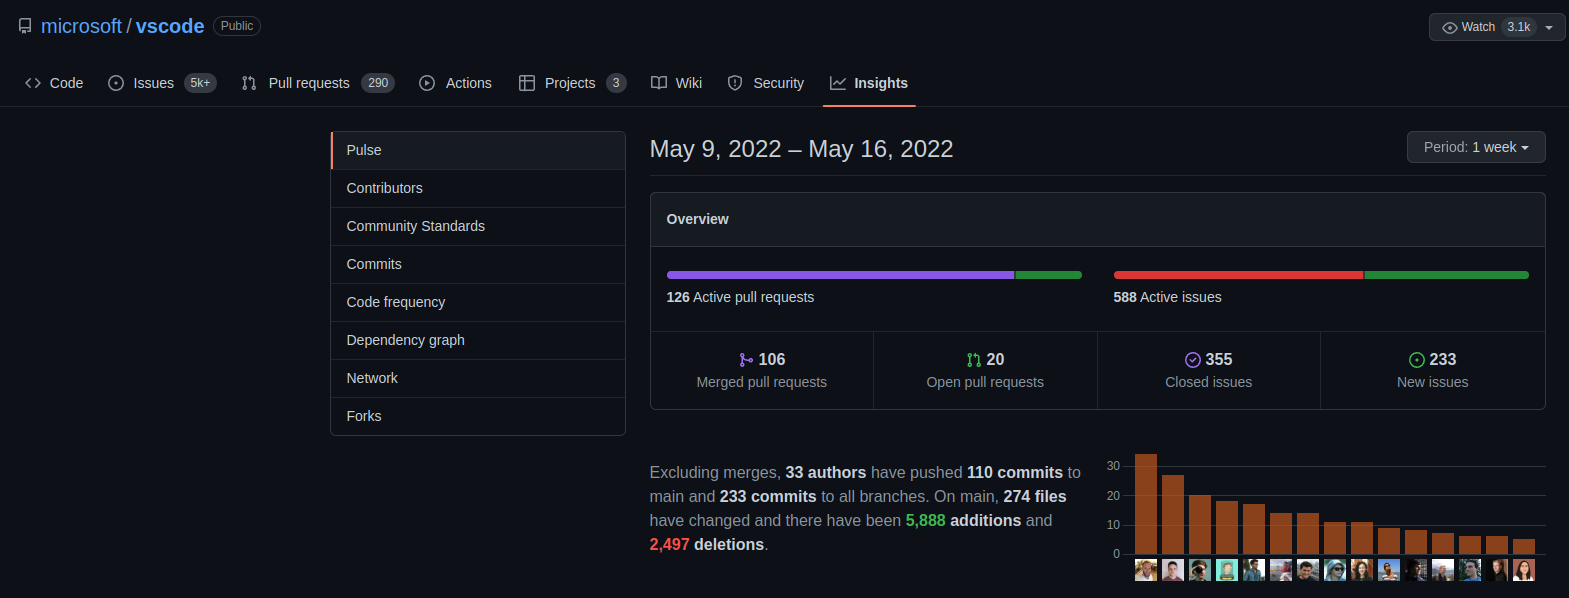
\includegraphics[width=1\textwidth]{GItHub-Insights.png}
  \caption{Ejemplo de la web de estadísticas en la página oficial de
    GitHub.}
  \label{figure:GithubInsights}
\end{figure}

En la figura~\ref{figure:GithubInsights} se muestra un ejemplo de un
ejemplo de un panel de estadísticas de los múltiples que ofrece GitHub,
como vemos, tienen una apariencia limpia y muy clara, con una interfaz
sencilla de usar y muy cómoda. Para el ejemplo se ha tomado el repositorio
de "vscode" de microsoft, como vemos es un repositorio público lo que
permite ver las estadísticas completas, como ya se ha comentado, en caso de
querer visualizarlas para un repositorio privado al cual tengamos acceso,
ya sea siendo propietarios del mismo o como colaborador, necesitaríamos
contar con una cuenta premium para poder visualizarlas, teniendo que
realizar un pago mensual para ello.

En la parte izquierda, podemos visualizar un menú seleccionable, en el cual
elegimos que estadísiticas queremos visualizar, ofreciendo distintas
posibilidades, siendo para el caso tratado las mas interesantes las
relacionadas con los commits, contribuidores y la frecuencia con la que se
ha programado.

\subsubsection{GitHub Education}

Github Education\footnote{\url{https://education.github.com}.}, de la mano
de GitHub, se ofrecen múltiples servicios de pago destinados a la
educación. Estos servicios son aplicables a distintas instituciones
educativas y de distintos tamaños. Estas pueden llegar a un convenio con
GitHub, contando con múltiples tipos de ayudas para la contratación de
servicios.

Entre los servicios distinguimos entre herramientas para el profesorado y
herramientas para el alumnado. Ofreciendo diferentes ventajas destinadas a
los requerimientos de cada uno. En este caso, el análisis está más enfocado
en cuanto a las ventajas que puede obtener el profesorado, a modo de
comparativa con la herramienta desarrollada, cuyo fín es el soporte a los
profesores para llevar el control de los alumnos.

Desde la página web de GitHub, encontramos una guía donde se indican
claramente los pasos que se han de seguir para darse de alta como profesor,
indicando que el proceso conlleva alrededor de unos 15 minutos, una vez
realizado el registro, se cuentan con las siguientes herramientas:
\begin{itemize}
\item Acceso a ``Education Community'', un lugar donde los educadores
  pueden comentar sus ideas acerca de las tendencias de la educación
  tecnológica. Pudiendo así comentar, investigar y aprender nuevas formas
  de comunicación, enseñanza y esquemas de trabajo para sus alumnos.
  Además, se pueden consultar dudas acerca de cualquier problema
  relacionado con el uso de las herramientas ofrecidas, contando con una
  amplia comunidad activa, que da solución a múltiples consultas y
  problemas.
\item Posibilidad de solicitar un ``botín de GitHub'', incluyendo este
  beneficios educativos y material destinado a los estudiantes. En caso de
  ser aprobada la solicitud, se reciben múltiples tutoriales y guías sobre
  el uso de Git, posters, stickers, y algunas tarjetas de regalo de
  camisetas de GitHub, canjeables por los alumnos en la web, destinados a
  ofrecer a modo de premio a los estudiantes con mejor desempeño.
\item Acceso a ``GitHub Teams'', permitiendo tener un número ilimitado de
  usuarios y repositorios privados.
\item El software completo de “GitHub classroom”, una aplicación web tanto para docentes como alumnos, que permite entre otras, (i) la creación de aulas virtuales, donde los alumnos y maestros interactúan a lo largo de la duración del curso. Un mismo profesor puede crear diferentes aulas virtuales donde se impartirán diferentes asignaturas posibles.(ii) Creación de tareas, tanto de manera individual como grupales, creandolas algún de los docentes con permiso en el aula y consiguiendo un enlace el cual los alumnos usarán para el acceso.~\ref{figure:GitHubClassroomTareas} (iii) Crear plantillas a partir de un
  repositorio inicial de tal forma que el código sea sencillamente
  distribuible a los alumnos. (iv) Programar tareas con una calificación
  automática, es decir, una vez los alumnos entregan la tarea, siguiendo
  las indicaciones asignadas a la tarea, esta se autoevalúan, teniendo
  acceso en tiempo real de parte de los alumnos de las calificaciones y
  haciendo más eficiente el trabajo del profesor.~\ref{figure:GitHubClassroomTareas} (v) Control total de los
  repositorios creados sobre el aula de trabajo, permitiendo, tanto
  comunicación con los alumnos, como un amplio catálogo de estadísticas y
  herramientas para la evaluación. Permitiendo la evaluación y corrección de los repositorios de los alumnos de forma rápida y sencilla, pudiendo realizar comentarios sobre los commits creados y teniendo interacción con los alumnos.
  \begin{figure}[h!]
    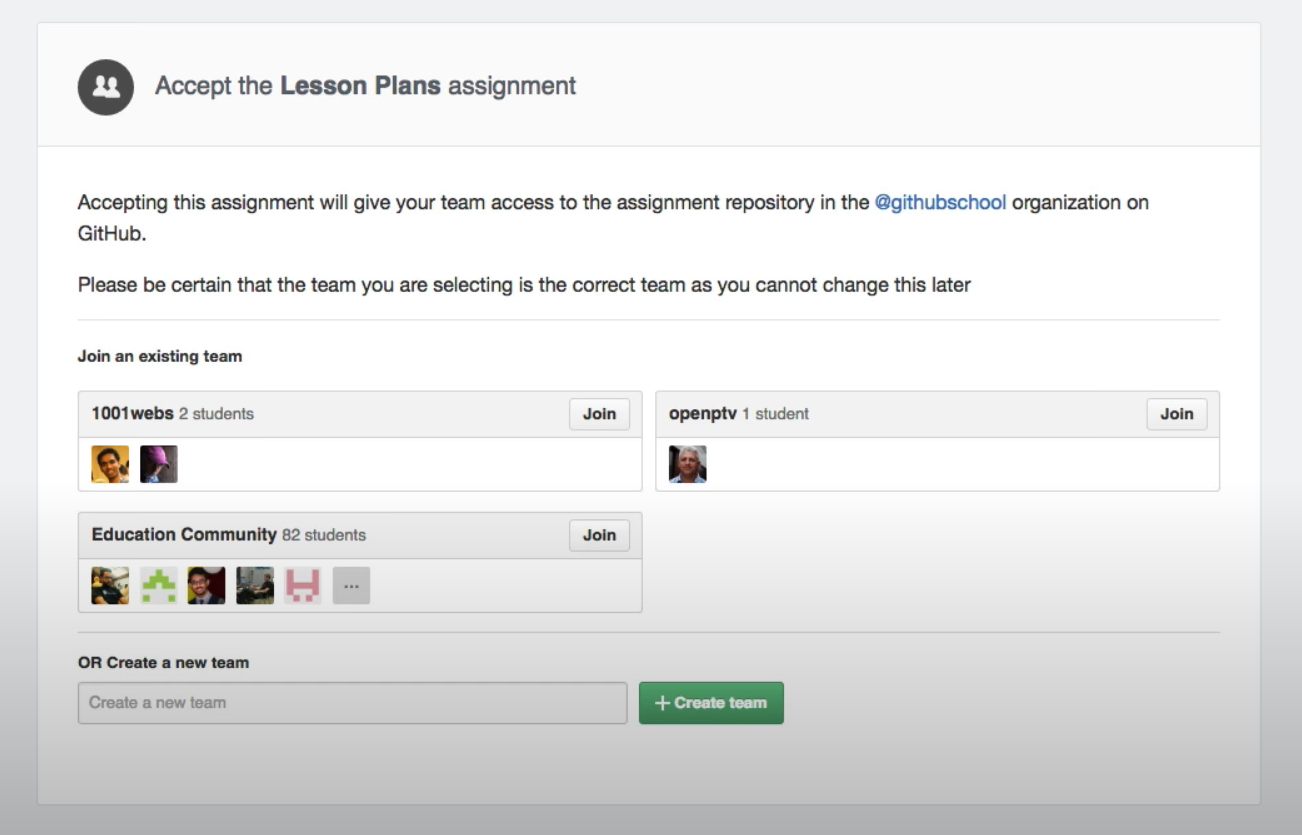
\includegraphics[width=1\textwidth]{GithubClassromEquipos.png}
    \caption{Panel de creación de tareas tanto individuales como en grupo, por parte del/los tutores.}
    \label{figure:GitHubClassroomTareas}
  \end{figure}
  \begin{figure}[h!]
    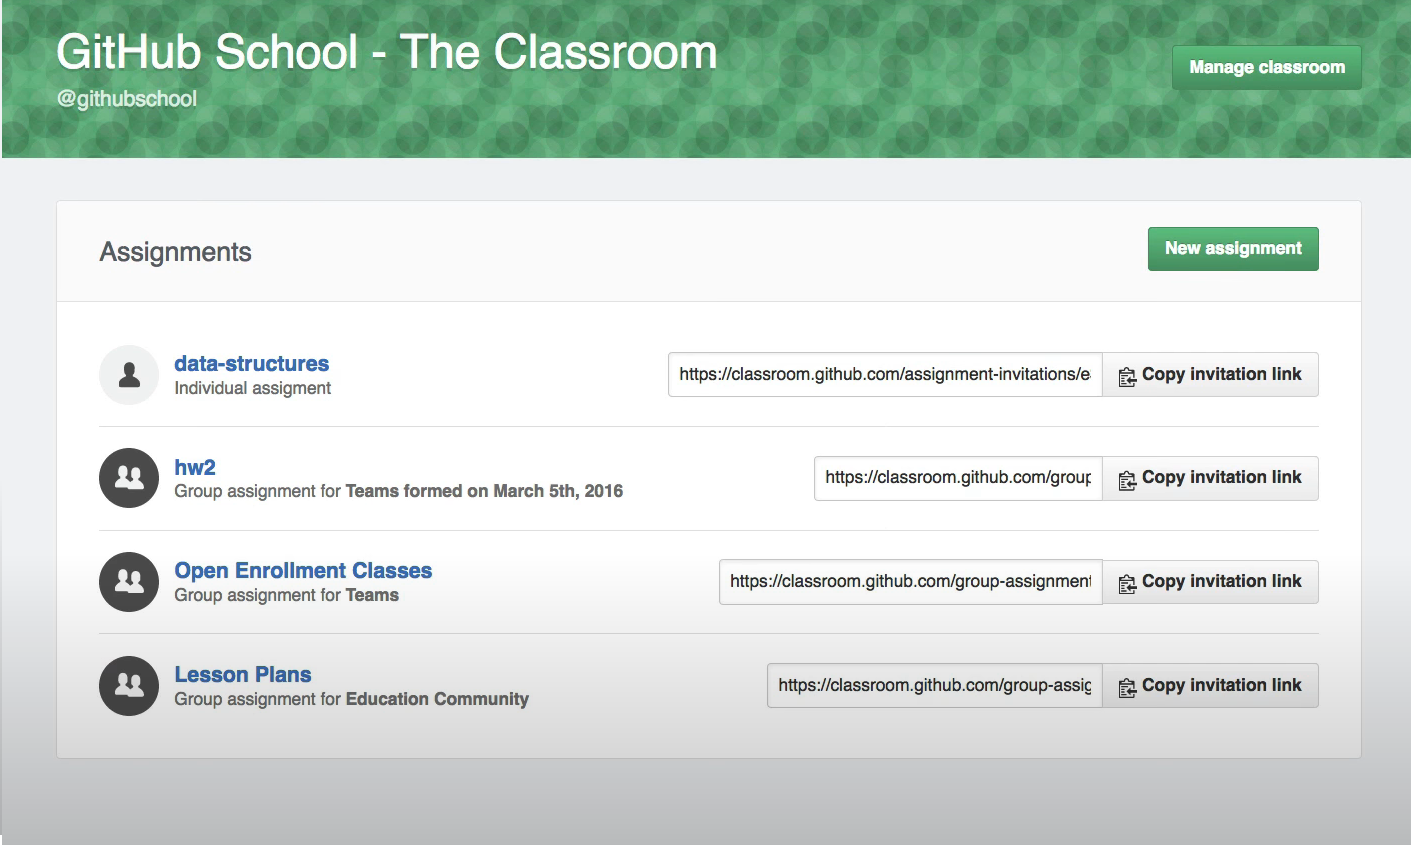
\includegraphics[width=1\textwidth]{GithubClassroomTareasIndividuales.png}
    \caption{Gestión de tareas grupales y creación de equipos por parte de los alumnos, gestionada automáticamente.}
    \label{figure:GitHubClassroomEquipos}
  \end{figure}

\item Solicitud de servicios cloud, aplicados a la enseñanza de nuevas
  tecnologías, contando con colaboradores de alta influencia en la
  actualidad de los servicios cloud, como lo son Digitalocean o Azure.
\end{itemize}

\subsection{Estadisticas de GitLab}

En el caso del proveedor GitLab, si se ofrece soporte para la consulta de
estadísticas de los repositorios, permitiendo ver gráficas sobre los
commits realizados, la distribución temporal de los mismos, además se
ofrecen datos acerca del ``coverage'' del código del repositorio, y
porcentajes de uso en caso de utilizarse más de un lenguaje de programación
sobre el proyecto.

\begin{figure}[h!]
  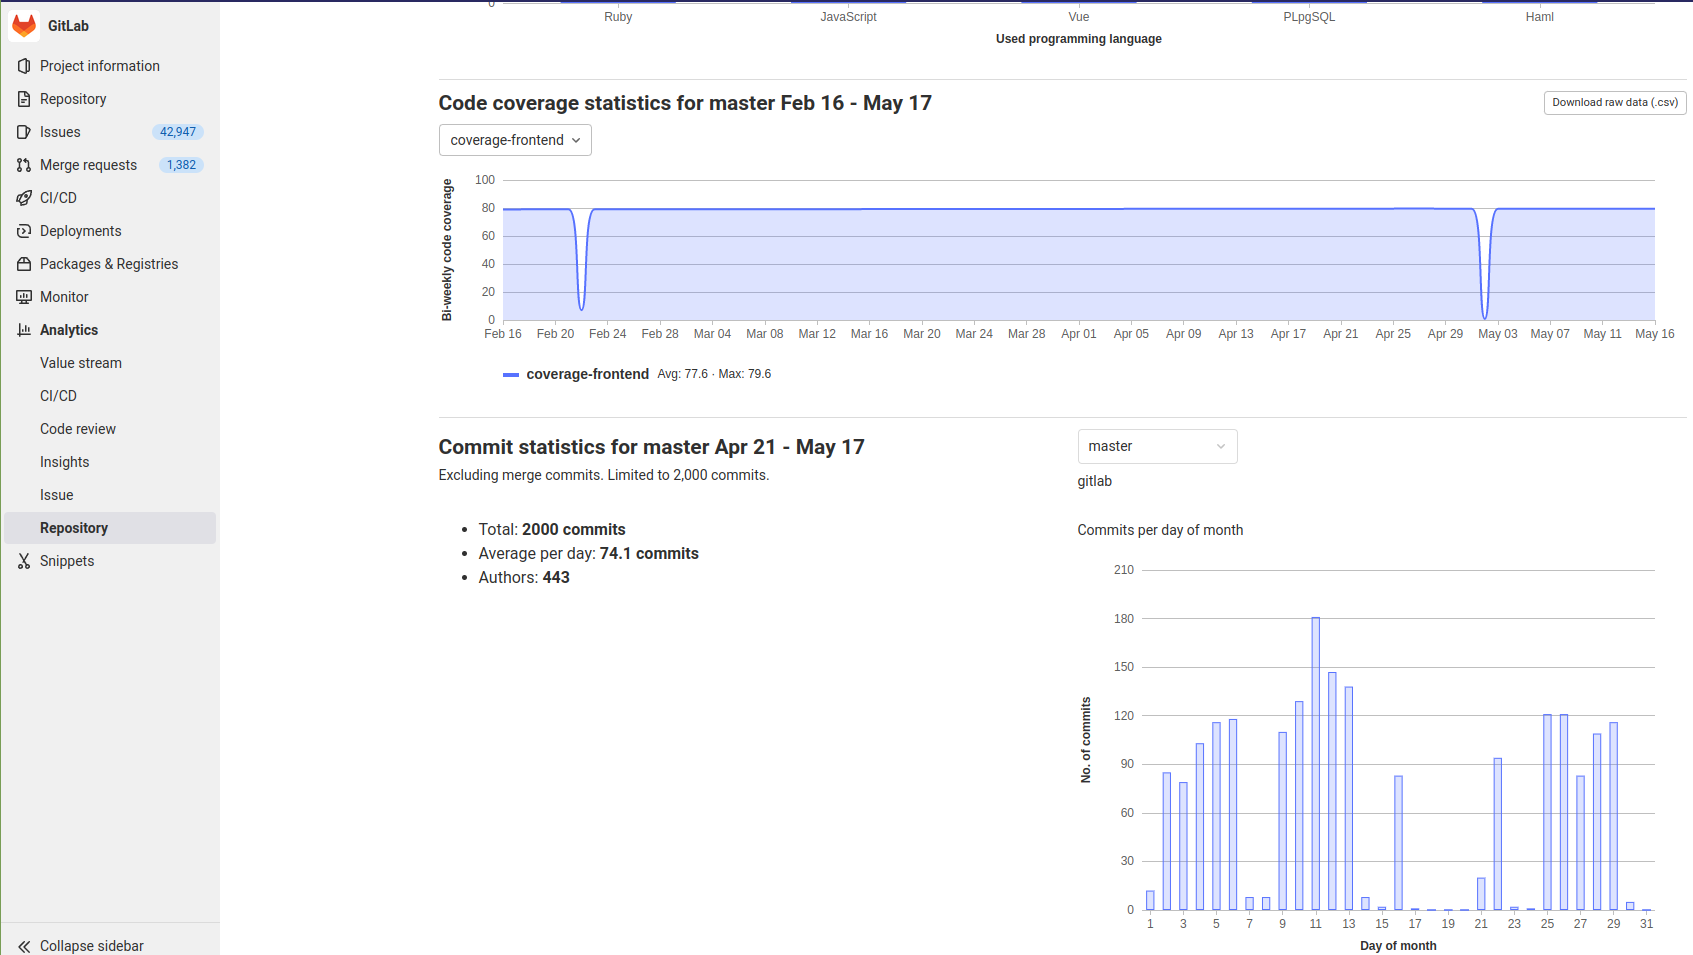
\includegraphics[width=\textwidth]{GitLab-stats.png}
  \caption{Ejemplo de la web de estadísticas en la página oficial de
    GitLab.}
  \label{figure:GitLabInsights}
\end{figure}

En la figura~\ref{figure:GitLabInsights}, se muestra una captura de la web
de GitLab, y mostrando información relacionada con un repositorio público,
podemos encontrar a la izquierda una sección en la que seleccionar las
diferentes analiticas ofrecidas para el repositorio.

Respecto a la accesibilidad de los datos, en el caso de la web de GitHub,
se muestran de forma más clara y accesible, conteniendo además datos de
mayor relevancia para el propósito que se está tratando y más cantidad de
información. En cuanto el posible uso del profesorado de GitLab para la
consulta de estadísticas, se destaca que el acceso a los repositorios, no
es el más rápido, en mayor instancia en caso de ser un número alto de
repositorios, pudiéndose hacer difícil y tedioso la consulta de todos
ellos.

\subsubsection{GitLab for education}

\textbf{GitLab for
  Education}\footnote{\url{https://about.gitlab.com/solutions/education/}.}:
Al igual que GitHub, GitLab también ofrece servicios destinados a la
educación, en este caso también son servicios de pago y como en el otro
caso, con posibilidad de solicitar múltiples tipos de subvenciones para la
institución donde se quiera aplicar el programa para la educación de
GitLab.

En cuanto a lo ofrecido, los principales objetivos del programa de
educación son: (i) Creación de cuentas para los usuarios de la institución
educativa sin límites. (ii) Colaboración entre profesorado y alumno. (iii)
Acceso al foro de GitLab con categorías específicas para la educación y un
amplio catálogo de miembros. (iv) Guias para el alumnado sobre las
tecnologías ofrecidas (v) Acceso a los eventos “Hackaton” donde los alumnos
pueden competir en jornadas de programación, colaborando con problemas de
la comunidad, y accediendo a un amplio número de premios para los mejores
contribuidores. (vi) Ofrece a los alumnos una visión del ciclo de vida DevOps, pudiendo aplicar sobre los repositorios integración y entrega continua, permitiendo así desarrollar, probar y desplegar el código de forma más sencilla. GitLab ofrece herramientas propias con las que se posibilita esta tarea y pudiendo realizar las pruebas en remoto, contando con 50000 minutos de CI/CD. 


En cuanto a las diferencias con GitHub education, ofrecen servicios que no
solo son válidos en la educación, ofreciendo distintos planes tanto para
empresas e instituciones de cualquier tipo. El servicio de GitHub está
plenamente enfocado en la educación, y ofrece un control al profesorado más
amplio que GitLab, permitiendo la creación de aula, tareas de distintos
tipos etc.


\subsection{Limitaciones de las herramientas existentes y ventajas de la
  herramienta implementada}

Las herramientas de analisis de repositorios en múltiples casos, como hemos
visto, requieren una suscripción de pago a un servicio, excepto en el caso
de GitLab en la que su panel de estadísticas si se ofrece de manera abierta
tanto para repositorios públicos y privados. Sin embargo, en los paneles de
estadísticas ofrecidos por ambos proveedores, no se muestra de forma rápida
el contenido de los commits, teniendo que acceder previamente a los commits
y visualizarlos uno por uno, esto es un aspecto bastante negativo ya que
para la correción de los alumnos, es necesario visualizar el interior de
los commits, ya que en muchos casos estos pueden contener simples
modificaciones que realmente no conllevan un gran trabajo por parte de
dicho alumno, esto indica que únicamente con visualizar el numero de
commits de cada alumno y la distribución temporal de la misma no es
suficiente y es necesario visualizar el contenido de los mismos.
Encontramos por tanto, que el profesorado debe acceder por separado a los
commits y las estadísticas en las soluciones propuestas, esto repetido para
cada uno de sus alumnos.

Por otra parte, sobre los servicios ofrecidos especificamente para las
instituciones, son una gran oportunidad de integrar en la institución la
herramienta de Git, ofreciendo múltiples ventajas tanto para la misma
institución como para sus integrantes. Sin embargo, estas soluciones
requieren de un convenio entre la institución y el proveedor de servicios,
esto en muchos casos no es sencillo, conllevando múltiples gestiones y
requerimientos, además teniendo de tener en cuenta el coste que conlleva
para la institución la integración de dichos servicios.

Como conclusión, tras conocer diferentes alternativas válidas para el
control del trabajo realizado por parte del alumnado, podemos destacar los
siguientes beneficios de la herramienta desarrollada en este trabajo:

\begin{itemize}
\item Una herramienta libre de pagos, tanto por parte del profesorado como
  de la institución.
\item Control de los datos del profesorado, estos datos se manejan de forma
  interna en la institución de la universidad de Murcia, teniendo el
  control total de dichos datos, y no dependiendo de un servicio externo.
\item Herramienta desarrollada por la propia Facultad, con un margen de
  mejora muy amplio y posibilidad de implementar nuevas funcionalidades,
  que se adapten específicamente a las necesidades de la institución.
  Pudiendo además extrapolar a distintas facultades para la gestión de
  distintos proyectos.
\item Es un proyecto plenamente escalable, mediante el uso de contenedores
  Docker pudiendo ofrecer un buen rendimiento incluso bajo un nivel de
  requerimiento alto
\item Un acceso rápido y eficiente a las estadísticas de los repositorios
  de los alumnos, obteniendo la información necesaria con el menor número
  de ``clicks'' posible.
\end{itemize}

%%% Local variables:
%%% TeX-master: "memoria.tex"
%%% coding: utf-8
%%% ispell-local-dictionary: "spanish"
%%% TeX-parse-self: t
%%% TeX-auto-save: t
%%% fill-column: 75
%%% End:

%  LocalWords:  Scala interoperabilidad metamodelado metamodelo Ecore
%  LocalWords:  Sirius
